\documentclass[11pt,a4paper]{article}
\usepackage[margin=2cm]{geometry}
\usepackage[T1]{fontenc}
\usepackage[utf8]{inputenc}
\usepackage{mathptmx}
\usepackage{amsmath,amssymb}
\usepackage{booktabs}
\usepackage{tabularx}
\usepackage{graphicx}
\usepackage[table]{xcolor}
\usepackage{caption}
\usepackage{enumitem}
\usepackage{microtype}
\usepackage[hidelinks]{hyperref}

\captionsetup{font=small,labelfont=bf,skip=4pt}
\renewcommand{\topfraction}{0.9}
\renewcommand{\bottomfraction}{0.8}
\renewcommand{\textfraction}{0.07}
\renewcommand{\floatpagefraction}{0.85}
\setcounter{topnumber}{3}\setcounter{bottomnumber}{2}\setcounter{totalnumber}{5}
\setlength{\textfloatsep}{8pt plus 2pt minus 2pt}
\setlength{\floatsep}{6pt plus 2pt minus 2pt}
\setlength{\parskip}{3pt}
\setlength{\parindent}{0pt}
\setlist{nosep,leftmargin=1.2em}
\setlength{\tabcolsep}{4pt}
\renewcommand{\arraystretch}{1.12}
\newcommand{\st}{\ensuremath{{\scriptstyle\bigstar}}}
\newcommand{\pmstd}[2]{#1\,{\scriptsize$\pm$\,#2}}
% auto-generated by extract_explain_colors.py: one coloured box per word, colours taken from results/explain/*.png
\newcommand{\exbigruattention}{%
\colorbox[RGB]{252,204,183}{\strut i}\hspace{1.2pt}\allowbreak \colorbox[RGB]{225,46,38}{\strut \textcolor{white}{do}}\hspace{1.2pt}\allowbreak \colorbox[RGB]{252,149,117}{\strut n\textquoteright{}t}\hspace{1.2pt}\allowbreak \colorbox[RGB]{254,227,215}{\strut have}\hspace{1.2pt}\allowbreak \colorbox[RGB]{254,228,216}{\strut cravings}\hspace{1.2pt}\allowbreak \colorbox[RGB]{254,233,224}{\strut after}\hspace{1.2pt}\allowbreak \colorbox[RGB]{254,229,218}{\strut taking}\hspace{1.2pt}\allowbreak \colorbox[RGB]{254,231,221}{\strut this}\hspace{1.2pt}\allowbreak \colorbox[RGB]{254,231,220}{\strut at}\hspace{1.2pt}\allowbreak \colorbox[RGB]{254,233,223}{\strut night}\hspace{1.2pt}\allowbreak \colorbox[RGB]{254,229,218}{\strut !}\hspace{1.2pt}\allowbreak \colorbox[RGB]{254,232,222}{\strut i}\hspace{1.2pt}\allowbreak \colorbox[RGB]{254,232,222}{\strut \textquoteright{}m}\hspace{1.2pt}\allowbreak \colorbox[RGB]{103,0,12}{\strut \textcolor{white}{horrible}}\hspace{1.2pt}\allowbreak \colorbox[RGB]{253,208,189}{\strut with}\hspace{1.2pt}\allowbreak \colorbox[RGB]{254,227,214}{\strut eating}\hspace{1.2pt}\allowbreak \colorbox[RGB]{252,200,179}{\strut late}\hspace{1.2pt}\allowbreak \colorbox[RGB]{254,232,222}{\strut at}\hspace{1.2pt}\allowbreak \colorbox[RGB]{254,234,224}{\strut night}\hspace{1.2pt}\allowbreak \colorbox[RGB]{254,234,224}{\strut ,}\hspace{1.2pt}\allowbreak \colorbox[RGB]{254,235,225}{\strut i}\hspace{1.2pt}\allowbreak \colorbox[RGB]{254,228,216}{\strut do}\hspace{1.2pt}\allowbreak \colorbox[RGB]{254,232,222}{\strut it}\hspace{1.2pt}\allowbreak \colorbox[RGB]{254,233,223}{\strut almost}\hspace{1.2pt}\allowbreak \colorbox[RGB]{254,235,225}{\strut every}\hspace{1.2pt}\allowbreak \colorbox[RGB]{254,235,225}{\strut night}\hspace{1.2pt}\allowbreak \colorbox[RGB]{254,235,225}{\strut after}\hspace{1.2pt}\allowbreak \colorbox[RGB]{254,231,220}{\strut dinner}\hspace{1.2pt}\allowbreak \colorbox[RGB]{254,234,224}{\strut and}\hspace{1.2pt}\allowbreak \colorbox[RGB]{254,235,225}{\strut i}\hspace{1.2pt}\allowbreak \colorbox[RGB]{254,235,225}{\strut \textquoteright{}m}\hspace{1.2pt}\allowbreak \colorbox[RGB]{254,233,223}{\strut sure}\hspace{1.2pt}\allowbreak \colorbox[RGB]{254,233,224}{\strut it}\hspace{1.2pt}\allowbreak \colorbox[RGB]{254,233,223}{\strut \textquoteright{}s}\hspace{1.2pt}\allowbreak \colorbox[RGB]{254,232,222}{\strut part}\hspace{1.2pt}\allowbreak \colorbox[RGB]{254,234,224}{\strut of}\hspace{1.2pt}\allowbreak \colorbox[RGB]{254,233,224}{\strut the}\hspace{1.2pt}\allowbreak \colorbox[RGB]{253,220,205}{\strut reason}\hspace{1.2pt}\allowbreak \colorbox[RGB]{254,234,224}{\strut i}\hspace{1.2pt}\allowbreak \colorbox[RGB]{254,234,224}{\strut \textquoteright{}m}\hspace{1.2pt}\allowbreak \colorbox[RGB]{253,223,209}{\strut overweight}\hspace{1.2pt}\allowbreak \colorbox[RGB]{254,231,220}{\strut .}\hspace{1.2pt}\allowbreak \colorbox[RGB]{254,229,217}{\strut but}\hspace{1.2pt}\allowbreak \colorbox[RGB]{254,234,224}{\strut when}\hspace{1.2pt}\allowbreak \colorbox[RGB]{254,234,224}{\strut i}\hspace{1.2pt}\allowbreak \colorbox[RGB]{254,231,221}{\strut take}\hspace{1.2pt}\allowbreak \colorbox[RGB]{254,233,224}{\strut this}\hspace{1.2pt}\allowbreak \colorbox[RGB]{254,235,225}{\strut ,}\hspace{1.2pt}\allowbreak \colorbox[RGB]{254,233,224}{\strut the}\hspace{1.2pt}\allowbreak \colorbox[RGB]{253,214,197}{\strut cravings}\hspace{1.2pt}\allowbreak \colorbox[RGB]{254,233,223}{\strut are}\hspace{1.2pt}\allowbreak \colorbox[RGB]{253,207,188}{\strut gone}\hspace{1.2pt}\allowbreak \colorbox[RGB]{254,233,223}{\strut !}\hspace{1.2pt}\allowbreak \colorbox[RGB]{254,230,219}{\strut !}}
\newcommand{\exrobertaattention}{%
\colorbox[RGB]{254,225,212}{\strut I}\hspace{1.2pt}\allowbreak \colorbox[RGB]{254,233,224}{\strut don}\hspace{1.2pt}\allowbreak \colorbox[RGB]{253,218,202}{\strut \textquoteright{}}\hspace{1.2pt}\allowbreak \colorbox[RGB]{254,235,225}{\strut t}\hspace{1.2pt}\allowbreak \colorbox[RGB]{254,238,230}{\strut have}\hspace{1.2pt}\allowbreak \colorbox[RGB]{254,234,224}{\strut cravings}\hspace{1.2pt}\allowbreak \colorbox[RGB]{253,216,200}{\strut after}\hspace{1.2pt}\allowbreak \colorbox[RGB]{254,239,232}{\strut taking}\hspace{1.2pt}\allowbreak \colorbox[RGB]{254,231,221}{\strut this}\hspace{1.2pt}\allowbreak \colorbox[RGB]{254,239,231}{\strut at}\hspace{1.2pt}\allowbreak \colorbox[RGB]{254,241,234}{\strut night}\hspace{1.2pt}\allowbreak \colorbox[RGB]{251,131,99}{\strut !}\hspace{1.2pt}\allowbreak \colorbox[RGB]{254,234,224}{\strut I}\hspace{1.2pt}\allowbreak \colorbox[RGB]{254,229,218}{\strut \textquoteright{}}\hspace{1.2pt}\allowbreak \colorbox[RGB]{254,237,229}{\strut m}\hspace{1.2pt}\allowbreak \colorbox[RGB]{254,235,226}{\strut horrible}\hspace{1.2pt}\allowbreak \colorbox[RGB]{254,241,234}{\strut with}\hspace{1.2pt}\allowbreak \colorbox[RGB]{254,243,237}{\strut eating}\hspace{1.2pt}\allowbreak \colorbox[RGB]{254,243,237}{\strut late}\hspace{1.2pt}\allowbreak \colorbox[RGB]{254,240,233}{\strut at}\hspace{1.2pt}\allowbreak \colorbox[RGB]{254,242,236}{\strut night}\hspace{1.2pt}\allowbreak \colorbox[RGB]{254,241,234}{\strut ,}\hspace{1.2pt}\allowbreak \colorbox[RGB]{254,243,238}{\strut I}\hspace{1.2pt}\allowbreak \colorbox[RGB]{254,244,239}{\strut do}\hspace{1.2pt}\allowbreak \colorbox[RGB]{254,243,237}{\strut it}\hspace{1.2pt}\allowbreak \colorbox[RGB]{254,243,238}{\strut almost}\hspace{1.2pt}\allowbreak \colorbox[RGB]{254,243,238}{\strut every}\hspace{1.2pt}\allowbreak \colorbox[RGB]{254,243,237}{\strut night}\hspace{1.2pt}\allowbreak \colorbox[RGB]{254,244,239}{\strut after}\hspace{1.2pt}\allowbreak \colorbox[RGB]{254,243,238}{\strut dinner}\hspace{1.2pt}\allowbreak \colorbox[RGB]{254,242,236}{\strut and}\hspace{1.2pt}\allowbreak \colorbox[RGB]{254,243,238}{\strut I}\hspace{1.2pt}\allowbreak \colorbox[RGB]{254,239,232}{\strut \textquoteright{}}\hspace{1.2pt}\allowbreak \colorbox[RGB]{254,243,238}{\strut m}\hspace{1.2pt}\allowbreak \colorbox[RGB]{254,243,238}{\strut sure}\hspace{1.2pt}\allowbreak \colorbox[RGB]{254,242,236}{\strut it}\hspace{1.2pt}\allowbreak \colorbox[RGB]{254,238,230}{\strut \textquoteright{}}\hspace{1.2pt}\allowbreak \colorbox[RGB]{254,243,237}{\strut s}\hspace{1.2pt}\allowbreak \colorbox[RGB]{254,241,235}{\strut part}\hspace{1.2pt}\allowbreak \colorbox[RGB]{254,243,238}{\strut of}\hspace{1.2pt}\allowbreak \colorbox[RGB]{254,243,237}{\strut the}\hspace{1.2pt}\allowbreak \colorbox[RGB]{254,243,238}{\strut reason}\hspace{1.2pt}\allowbreak \colorbox[RGB]{254,241,234}{\strut I}\hspace{1.2pt}\allowbreak \colorbox[RGB]{254,235,225}{\strut \textquoteright{}}\hspace{1.2pt}\allowbreak \colorbox[RGB]{254,241,234}{\strut m}\hspace{1.2pt}\allowbreak \colorbox[RGB]{254,239,232}{\strut overweight}\hspace{1.2pt}\allowbreak \colorbox[RGB]{103,0,12}{\strut \textcolor{white}{.}}\hspace{1.2pt}\allowbreak \colorbox[RGB]{253,219,203}{\strut But}\hspace{1.2pt}\allowbreak \colorbox[RGB]{254,231,220}{\strut when}\hspace{1.2pt}\allowbreak \colorbox[RGB]{254,235,225}{\strut I}\hspace{1.2pt}\allowbreak \colorbox[RGB]{254,239,231}{\strut take}\hspace{1.2pt}\allowbreak \colorbox[RGB]{254,229,217}{\strut this}\hspace{1.2pt}\allowbreak \colorbox[RGB]{254,233,223}{\strut ,}\hspace{1.2pt}\allowbreak \colorbox[RGB]{254,235,225}{\strut the}\hspace{1.2pt}\allowbreak \colorbox[RGB]{254,234,224}{\strut cravings}\hspace{1.2pt}\allowbreak \colorbox[RGB]{254,237,228}{\strut are}\hspace{1.2pt}\allowbreak \colorbox[RGB]{254,237,228}{\strut gone}\hspace{1.2pt}\allowbreak \colorbox[RGB]{252,158,128}{\strut !!}}
\newcommand{\exrobertaocclusion}{%
\colorbox[RGB]{248,239,234}{\strut I}\hspace{1.2pt}\allowbreak \colorbox[RGB]{225,236,243}{\strut don}\hspace{1.2pt}\allowbreak \colorbox[RGB]{250,232,221}{\strut \textquoteright{}}\hspace{1.2pt}\allowbreak \colorbox[RGB]{250,232,221}{\strut t}\hspace{1.2pt}\allowbreak \colorbox[RGB]{248,193,166}{\strut have}\hspace{1.2pt}\allowbreak \colorbox[RGB]{226,237,243}{\strut cravings}\hspace{1.2pt}\allowbreak \colorbox[RGB]{250,232,221}{\strut after}\hspace{1.2pt}\allowbreak \colorbox[RGB]{122,182,214}{\strut taking}\hspace{1.2pt}\allowbreak \colorbox[RGB]{223,236,242}{\strut this}\hspace{1.2pt}\allowbreak \colorbox[RGB]{249,234,225}{\strut at}\hspace{1.2pt}\allowbreak \colorbox[RGB]{248,191,163}{\strut night}\hspace{1.2pt}\allowbreak \colorbox[RGB]{192,53,56}{\strut \textcolor{white}{!}}\hspace{1.2pt}\allowbreak \colorbox[RGB]{164,206,227}{\strut I}\hspace{1.2pt}\allowbreak \colorbox[RGB]{241,244,246}{\strut \textquoteright{}}\hspace{1.2pt}\allowbreak \colorbox[RGB]{239,155,122}{\strut m}\hspace{1.2pt}\allowbreak \colorbox[RGB]{170,21,41}{\strut \textcolor{white}{horrible}}\hspace{1.2pt}\allowbreak \colorbox[RGB]{251,224,208}{\strut with}\hspace{1.2pt}\allowbreak \colorbox[RGB]{252,222,204}{\strut eating}\hspace{1.2pt}\allowbreak \colorbox[RGB]{214,231,241}{\strut late}\hspace{1.2pt}\allowbreak \colorbox[RGB]{247,246,246}{\strut at}\hspace{1.2pt}\allowbreak \colorbox[RGB]{251,227,214}{\strut night}\hspace{1.2pt}\allowbreak \colorbox[RGB]{251,227,214}{\strut ,}\hspace{1.2pt}\allowbreak \colorbox[RGB]{247,243,240}{\strut I}\hspace{1.2pt}\allowbreak \colorbox[RGB]{249,234,225}{\strut do}\hspace{1.2pt}\allowbreak \colorbox[RGB]{243,245,246}{\strut it}\hspace{1.2pt}\allowbreak \colorbox[RGB]{229,238,243}{\strut almost}\hspace{1.2pt}\allowbreak \colorbox[RGB]{248,242,238}{\strut every}\hspace{1.2pt}\allowbreak \colorbox[RGB]{238,243,245}{\strut night}\hspace{1.2pt}\allowbreak \colorbox[RGB]{238,243,245}{\strut after}\hspace{1.2pt}\allowbreak \colorbox[RGB]{231,239,244}{\strut dinner}\hspace{1.2pt}\allowbreak \colorbox[RGB]{217,233,241}{\strut and}\hspace{1.2pt}\allowbreak \colorbox[RGB]{234,241,244}{\strut I}\hspace{1.2pt}\allowbreak \colorbox[RGB]{240,243,245}{\strut \textquoteright{}}\hspace{1.2pt}\allowbreak \colorbox[RGB]{252,220,200}{\strut m}\hspace{1.2pt}\allowbreak \colorbox[RGB]{248,239,234}{\strut sure}\hspace{1.2pt}\allowbreak \colorbox[RGB]{244,245,246}{\strut it}\hspace{1.2pt}\allowbreak \colorbox[RGB]{238,243,245}{\strut \textquoteright{}}\hspace{1.2pt}\allowbreak \colorbox[RGB]{238,243,245}{\strut s}\hspace{1.2pt}\allowbreak \colorbox[RGB]{247,244,242}{\strut part}\hspace{1.2pt}\allowbreak \colorbox[RGB]{243,245,246}{\strut of}\hspace{1.2pt}\allowbreak \colorbox[RGB]{248,242,238}{\strut the}\hspace{1.2pt}\allowbreak \colorbox[RGB]{250,232,221}{\strut reason}\hspace{1.2pt}\allowbreak \colorbox[RGB]{243,245,246}{\strut I}\hspace{1.2pt}\allowbreak \colorbox[RGB]{237,242,245}{\strut \textquoteright{}}\hspace{1.2pt}\allowbreak \colorbox[RGB]{250,228,215}{\strut m}\hspace{1.2pt}\allowbreak \colorbox[RGB]{249,236,229}{\strut overweight}\hspace{1.2pt}\allowbreak \colorbox[RGB]{217,233,241}{\strut .}\hspace{1.2pt}\allowbreak \colorbox[RGB]{119,180,213}{\strut But}\hspace{1.2pt}\allowbreak \colorbox[RGB]{242,160,126}{\strut when}\hspace{1.2pt}\allowbreak \colorbox[RGB]{220,234,242}{\strut I}\hspace{1.2pt}\allowbreak \colorbox[RGB]{232,240,244}{\strut take}\hspace{1.2pt}\allowbreak \colorbox[RGB]{244,168,134}{\strut this}\hspace{1.2pt}\allowbreak \colorbox[RGB]{250,231,219}{\strut ,}\hspace{1.2pt}\allowbreak \colorbox[RGB]{228,238,243}{\strut the}\hspace{1.2pt}\allowbreak \colorbox[RGB]{217,233,241}{\strut cravings}\hspace{1.2pt}\allowbreak \colorbox[RGB]{252,220,200}{\strut are}\hspace{1.2pt}\allowbreak \colorbox[RGB]{103,0,31}{\strut \textcolor{white}{gone}}\hspace{1.2pt}\allowbreak \colorbox[RGB]{201,70,65}{\strut \textcolor{white}{!!}}}


\begin{document}

\begin{center}
{\large\bfseries DSL 504 --- Natural Language Processing \quad$\cdot$\quad Group Assignment 2, Question 2}\\[4pt]
{\LARGE\bfseries Fine-Tuning RoBERTa vs.\ a BiGRU + Attention Baseline\\[2pt] for 5-Class Amazon Review Rating Prediction}\\[6pt]
{\normalsize Agastya Nath \quad$\cdot$\quad Roll No.\ 12340140}
\end{center}



\section{Task and data}
\textbf{Dataset.} \texttt{SetFit/amazon\_reviews\_multi\_en} (English part of the Multilingual Amazon Reviews Corpus) with its official splits: 200{,}000 training, 5{,}000 validation and 5{,}000 test reviews. Every star rating makes up 20\% of each split, so the task is balanced 5-way classification. The validation set is used for early stopping and model selection only; each trained model is evaluated on the test set exactly once, using its best-validation checkpoint.

\textbf{Title + body.} The SetFit copy contains only the review body, so we recover each title from the MTEB copy of the same corpus (\texttt{mteb/AmazonReviewsClassification}, stored as ``title\textbackslash nbody'') by matching the whitespace-normalised body. Titles were found for \textbf{99.6\%} of training and 99.7\% of validation and test reviews (the rest use the body alone). The input is \textit{title}\,+\,``.~''\,+\,\textit{body}. The MTEB copy supplies only titles; all reviews, labels and splits come from the SetFit dataset.

\textbf{Metrics.} Accuracy, macro-F1, per-class F1 and the mean absolute error (MAE) between predicted and true stars. All results are the mean $\pm$ sample standard deviation over two seeds (42 and 13).

\section{Preprocessing}
\textbf{Classic pipeline (baseline).} HTML entities are unescaped, HTML tags and URLs are removed, and the text is lower-cased. We tokenize with spaCy's rule-based English tokenizer, which splits contractions (\textit{don't}~$\rightarrow$~\textit{do}, \textit{n't}) the way the embedding vocabulary does. The vocabulary is built from the training split only, keeping words seen at least 3 times, plus \texttt{<pad>} and \texttt{<unk>}. Sequences are truncated to 200 tokens. The embedding matrix is filled from fastText \texttt{wiki-news-300d-1M} vectors (cased vectors folded to lower case); words without a vector receive small random vectors, and \texttt{<pad>} is zero.

\textbf{RoBERTa pipeline.} \texttt{RobertaTokenizerFast} applies byte-level BPE and adds \texttt{<s>} \dots\ \texttt{</s>}; sequences are truncated to 256 sub-words (keeping \texttt{</s>}). Nothing is padded in advance: a \texttt{DataCollatorWithPadding} pads each batch to its own longest review (rounded up to a multiple of 8) and builds the \texttt{attention\_mask}. Batches are drawn from a length-bucketed sampler (shuffle, then group reviews of similar length). This reduces the token positions processed per epoch from 51.2\,M (fixed padding to 256) to 35.1\,M (dynamic padding) and to 10.9\,M with bucketing, raising the share of real tokens from 19\% to 89\%. The baseline uses the same sampler and per-batch padding.

\begin{table}[htbp]
\centering\small
\caption{Preprocessing statistics (training split unless noted).}
\label{tab:prep}
\begin{tabular}{lll}
\toprule
 & \textbf{Classic (BiGRU)} & \textbf{RoBERTa} \\
\midrule
Tokenization & spaCy word tokens & byte-level BPE \\
Vocabulary & 26{,}126 (min.\ freq.\ 3, from 50{,}197 types) & 50{,}265 (pre-trained) \\
Length: mean / 95th percentile & 44.6 / 117 tokens & 48.9 / 124 sub-words \\
Truncated reviews & 0.93\% (max 200) & 0.44\% (max 256) \\
Unknown tokens & 0.35\% of tokens (0.52\% on test) & none (byte fallback) \\
Pre-trained part & fastText: 96.2\% of types, 98.4\% of tokens covered & all 124\,M weights \\
\bottomrule
\end{tabular}
\end{table}

\section{Models}
\textbf{Baseline: BiGRU + additive attention pooling.} A 300-d embedding layer initialised with fastText (frozen during the first epoch, trainable afterwards; dropout 0.25) feeds a 2-layer bidirectional GRU with 256 units per direction (inter-layer dropout 0.3). Padded sequences are packed, so the backward GRU starts at each review's last real token. With $\mathbf{h}_t=[\overrightarrow{\mathbf{h}}_t;\overleftarrow{\mathbf{h}}_t]\in\mathbb{R}^{512}$ and mask $m_t$, additive attention pools the sequence:
\begin{equation*}
e_t=\mathbf{v}^{\top}\tanh(\mathbf{W}\mathbf{h}_t+\mathbf{b}),\qquad
\alpha_t=\frac{m_t\exp(e_t)}{\sum_j m_j\exp(e_j)},\qquad
\mathbf{c}=\sum_t\alpha_t\mathbf{h}_t ,
\end{equation*}
with $\mathbf{W}\in\mathbb{R}^{256\times512}$. Then come dropout (0.5) and a linear layer to 5 logits. The model has 10.0\,M parameters, 7.8\,M of them in the embedding table.

\textbf{RoBERTa with masked mean pooling.} We load the pre-trained \texttt{RobertaModel} (\texttt{roberta-base}: 12 layers, hidden size 768, 12 heads) without its pooler. The last hidden states $\mathbf{h}_t$ are averaged over the non-padded positions,
$\bar{\mathbf{h}}=\sum_t m_t\mathbf{h}_t\big/\sum_t m_t$,
followed by dropout (0.1) and a linear layer (768\,$\rightarrow$\,5). All 124.1\,M parameters are fine-tuned. For the ablation, $\bar{\mathbf{h}}$ is replaced by the first-token vector $\mathbf{h}_{\texttt{<s>}}$.

\section{Training setup}
Both models minimise cross-entropy. Table~\ref{tab:train} lists the settings. Validation macro-F1 is checked once per epoch for the baseline and four times per epoch for RoBERTa; training stops after a fixed number of checks without improvement, and the best checkpoint is restored before testing. Random seeds are fixed for Python, NumPy and PyTorch. All runs used one NVIDIA T4 GPU on Google Colab.

\begin{table}[htbp]
\centering\small
\caption{Training configuration.}
\label{tab:train}
\begin{tabular}{lll}
\toprule
 & \textbf{BiGRU + attention} & \textbf{RoBERTa} \\
\midrule
Optimiser & Adam, lr $10^{-3}$ & AdamW, lr $2\cdot10^{-5}$, $\beta=(0.9,0.98)$, $\epsilon=10^{-6}$ \\
Weight decay & -- & 0.01 (not on biases / LayerNorm) \\
LR schedule & constant & linear warm-up (6\%, 750 steps), then linear decay to 0 \\
Batch size / max.\ epochs & 128 / 10 & 32 / 2 (12{,}500 steps) \\
Early stopping & val.\ macro-F1, patience 2 epochs & val.\ macro-F1, patience 4 checks \\
Gradient clipping & max norm 1.0 & max norm 1.0 \\
Precision & fp16 autocast & fp16 autocast with loss scaling \\
Training time per run & 2.3 min & 26.9 min \\
\bottomrule
\end{tabular}
\end{table}

\section{Results}
\begin{table}[htbp]
\centering\small
\caption{Main results (mean $\pm$ std over seeds 42 and 13).}
\label{tab:main}
\begin{tabular}{lccccc}
\toprule
\textbf{Model} & \textbf{Test acc.\ (\%)} & \textbf{Test macro-F1 (\%)} & \textbf{Test MAE (stars)} & \textbf{Val.\ macro-F1 (\%)} & \textbf{Params} \\
\midrule
BiGRU + attention & \pmstd{63.72}{0.31} & \pmstd{63.65}{0.36} & \pmstd{0.426}{0.000} & \pmstd{63.42}{0.22} & 10.0\,M \\
RoBERTa (mean pooling) & \pmstd{\textbf{66.82}}{0.23} & \pmstd{\textbf{66.70}}{0.15} & \pmstd{\textbf{0.373}}{0.001} & \pmstd{66.32}{0.05} & 124.1\,M \\
\bottomrule
\end{tabular}
\end{table}

\textbf{Overall.} RoBERTa improves accuracy by 3.1 points, macro-F1 by 3.1 points and MAE by 12\% (Table~\ref{tab:main}). The gain is consistent: both RoBERTa runs (66.98\% and 66.66\% accuracy) beat both baseline runs (63.94\% and 63.50\%), and the seed-to-seed spread is about ten times smaller than the gap. The price is 12$\times$ more parameters and roughly 12$\times$ more training time.

\begin{figure}[htbp]
\centering
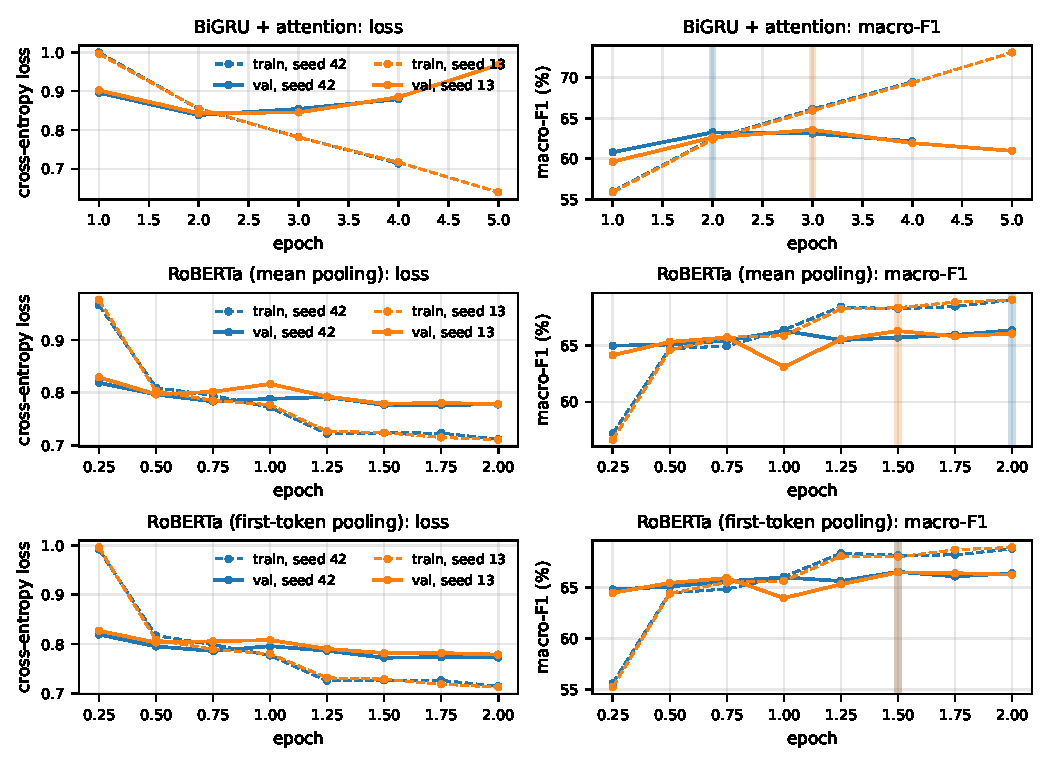
\includegraphics[width=\textwidth]{figures/fig_curves.pdf}
\caption{Training (dashed) and validation (solid) loss and macro-F1 for both seeds of every model; the bottom row is the first-token pooling ablation (Section~\ref{sec:ablation}). Training values are averaged over the batches since the previous check, with dropout active. Shaded bands mark the restored checkpoints.}
\label{fig:curves}
\end{figure}

\textbf{Training dynamics (Fig.~\ref{fig:curves}).} The baseline's validation loss is lowest after epoch 2, one epoch after the embeddings are unfrozen. Afterwards the training loss keeps falling while the validation loss rises, a clear sign of overfitting; early stopping ends training after 4--5 epochs and restores the epoch-2/3 checkpoints. RoBERTa already reaches 64--65\% validation macro-F1 after a quarter of an epoch, thanks to its pre-training, and then levels off around 66\%. In the second epoch its training loss (0.71) drops well below the validation loss (0.78) while validation F1 barely moves, so two epochs are enough. The best checkpoints occur at 1.5 and 2.0 epochs.

\begin{table}[htbp]
\centering\small
\caption{Per-class F1 and ordinal error profile on the test set (mean $\pm$ std over two seeds).}
\label{tab:perclass}
\setlength{\tabcolsep}{3pt}
\begin{tabular}{lccccc|ccc}
\toprule
 & \multicolumn{5}{c|}{\textbf{F1 per class (\%)}} & \textbf{Off by} & \textbf{Adjacent} & \textbf{1$\leftrightarrow$5} \\
\textbf{Model} & 1\,\st{} & 2\,\st{} & 3\,\st{} & 4\,\st{} & 5\,\st{} & $\geq$\textbf{2 (\%)} & \textbf{errors (\%)} & \textbf{(of 5{,}000)} \\
\midrule
BiGRU & \pmstd{71.0}{0.3} & \pmstd{54.7}{0.0} & \pmstd{54.7}{1.2} & \pmstd{60.0}{0.4} & \pmstd{77.8}{0.1} & \pmstd{5.33}{0.30} & \pmstd{85.3}{0.9} & \pmstd{10.0}{0.0} \\
RoBERTa & \pmstd{74.4}{0.0} & \pmstd{58.4}{0.5} & \pmstd{57.7}{0.4} & \pmstd{63.2}{0.5} & \pmstd{79.8}{0.4} & \pmstd{3.56}{0.08} & \pmstd{89.3}{0.3} & \pmstd{6.5}{0.7} \\
\bottomrule
\end{tabular}
\end{table}

\textbf{Per class.} RoBERTa wins on every class (Table~\ref{tab:perclass}, Fig.~\ref{fig:bars} left). For both models the extreme ratings are easiest (5\st{} $\approx$\,78--80 F1, 1\st{} $\approx$\,71--74) and the middle ratings hardest (2\st{} and 3\st{} $\approx$\,55--58). Reviews at the ends of the scale use strong, unambiguous language, while 2--4-star reviews mix praise and complaints, and different writers map the same opinion to neighbouring stars.

\begin{figure}[htbp]
\centering
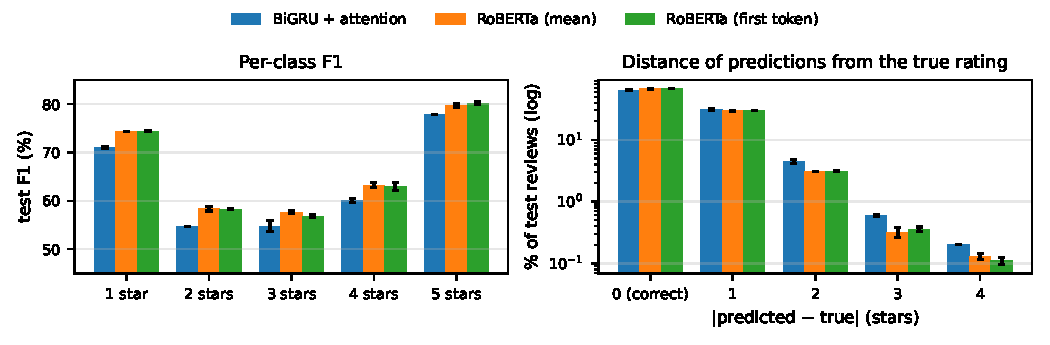
\includegraphics[width=\textwidth]{figures/fig_bars.pdf}
\caption{Left: test F1 per class. Right: share of test reviews by distance between predicted and true rating (log scale; 0 = correct). Error bars: std over two seeds.}
\label{fig:bars}
\end{figure}

\begin{figure}[htbp]
\centering
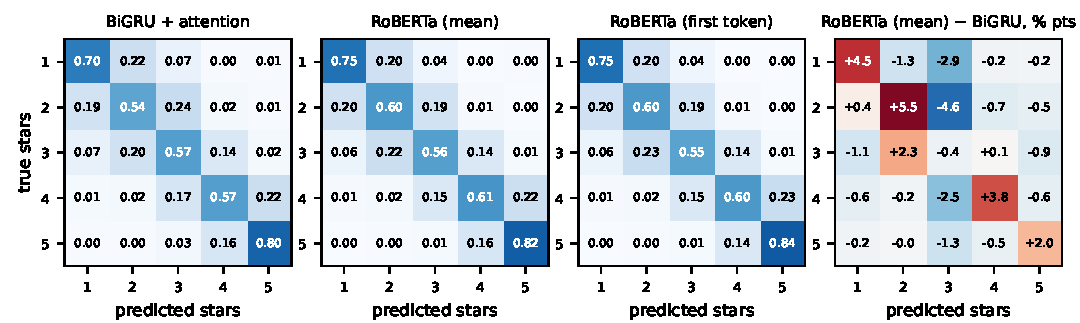
\includegraphics[width=\textwidth]{figures/fig_confusion.pdf}
\caption{Row-normalised test confusion matrices (both seeds pooled; the diagonal is per-class recall) for the baseline, RoBERTa and the first-token ablation, and the difference RoBERTa (mean) $-$ BiGRU in percentage points: red on the diagonal = higher recall for RoBERTa, blue off the diagonal = confusions RoBERTa makes less often.}
\label{fig:cm}
\end{figure}

\textbf{Adjacent vs.\ distant errors (Fig.~\ref{fig:cm}).} Almost all mistakes are one star off: 85\% of the baseline's errors and 89\% of RoBERTa's. Distant confusions are rare (Fig.~\ref{fig:bars} right). The share of reviews predicted $\geq$2 stars away falls from 5.3\% to 3.6\%, and 1$\leftrightarrow$5 confusions fall from 10 to 6.5 per 5{,}000 reviews; this is why MAE improves more (12\%) than accuracy (5\% relative). The difference panel shows that RoBERTa mostly gains recall on 2\st{} (+5.5 points), 1\st{} (+4.5) and 4\st{} (+3.8), mainly by no longer pushing these reviews towards 3 stars. Recall on 3\st{} itself is unchanged (56--57\%); its F1 still rises because fewer 2\st{} and 4\st{} reviews are wrongly labelled 3\st{}. The 4-vs-5 boundary stays hard: 22\% of 4-star reviews are predicted as 5 by both models, and the 4$\leftrightarrow$5 confusion rate barely moves (19.4\% vs.\ 18.9\%). This boundary often depends on small details and personal rating habits rather than on the review's sentiment.

\section{Ablation: mean pooling vs.\ first-token pooling}\label{sec:ablation}
We retrained RoBERTa with the first-token (\texttt{<s>}) vector instead of the masked mean, keeping everything else identical (two seeds).

\begin{table}[htbp]
\centering\small
\caption{Pooling ablation for RoBERTa (mean $\pm$ std over two seeds). Decisions are based on the validation columns.}
\label{tab:ablation}
\begin{tabular}{lcccccc}
\toprule
\textbf{Pooling} & \textbf{Val.\ macro-F1} & \textbf{Val.\ acc.} & \textbf{Val.\ MAE} & \textbf{Test macro-F1} & \textbf{Test acc.} & \textbf{Test MAE} \\
\midrule
Mean (main model) & \pmstd{66.32}{0.05} & \pmstd{66.44}{0.14} & \pmstd{0.378}{0.002} & \pmstd{66.70}{0.15} & \pmstd{66.82}{0.23} & \pmstd{0.373}{0.001} \\
First token \texttt{<s>} & \pmstd{66.51}{0.04} & \pmstd{66.69}{0.16} & \pmstd{0.375}{0.003} & \pmstd{66.50}{0.19} & \pmstd{66.70}{0.06} & \pmstd{0.375}{0.002} \\
\bottomrule
\end{tabular}
\end{table}

The two variants are practically equivalent (Table~\ref{tab:ablation}). First-token pooling is 0.19 points better on validation macro-F1, but mean pooling is 0.20 points better on test, so the ranking flips between two sets of 5{,}000 reviews. Their confusion matrices (Fig.~\ref{fig:cm}), per-class F1 and error profiles (Fig.~\ref{fig:bars}) and learning curves (Fig.~\ref{fig:curves}, bottom row) are also nearly identical, and both reach their best checkpoint after 1.5--2 epochs. Mean pooling would be expected to help when the useful information is spread over long inputs. Here reviews are short (median 38 sub-words), and because the whole network is fine-tuned, the \texttt{<s>} vector learns to summarise the review just as well. We keep mean pooling as the main model, as specified, and conclude that the pooling choice does not matter for this task.

\section{Qualitative analysis}
\textbf{Where the models disagree.} On the test set (seed 42), both models are right on 2{,}871 reviews (57.4\%) and both wrong on 1{,}325 (26.5\%). Only RoBERTa is right on 478 reviews (9.6\%) and only the baseline on 326 (6.5\%), a net gain of 152 reviews. To look for patterns, every test review was tagged with simple keyword rules (Table~\ref{tab:tags}). Three phenomena are clearly over-represented where only RoBERTa is right: reviews whose sentiment words point the wrong way (7.6\% of all reviews vs.\ 13.8\%, e.g.\ only negative words in a 4--5-star review), negation (52.8\% vs.\ 62.3\%) and contrast words such as \textit{but} or \textit{however} (38.8\% vs.\ 47.3\%). These all require reading words in context rather than counting them. The rules are only indicators. In particular, the ``sarcasm cue'' rule mostly fires on emphatic ``!!'' in sincere reviews, so we draw no conclusion about sarcasm.

\begin{table}[htbp]
\centering\small
\caption{Share of test reviews (\%) showing each heuristically tagged phenomenon, by which model is correct (seed 42).}
\label{tab:tags}
\begin{tabular}{lcccc}
\toprule
\textbf{Phenomenon (keyword rule)} & \textbf{All test} & \textbf{Only RoBERTa right} & \textbf{Only BiGRU right} & \textbf{Both wrong} \\
\midrule
Polarity mismatch (sentiment words vs.\ rating) & 7.6 & \textbf{13.8} & 4.6 & 11.8 \\
Negation (\textit{not, no, never, n't}, \dots) & 52.8 & \textbf{62.3} & 54.9 & 55.4 \\
Contrast (\textit{but, however, although}, \dots) & 38.8 & \textbf{47.3} & 45.7 & 45.4 \\
Mixed sentiment (positive and negative words) & 13.6 & 17.6 & 14.7 & 15.7 \\
Several \texttt{<unk>} tokens for the baseline & 4.6 & 5.6 & 5.2 & 5.7 \\
Very short ($\leq$8 words) & 7.2 & 3.3 & 4.9 & 4.4 \\
Sarcasm cue (\textit{wow, yeah right}, ``!!'', \dots) & 5.8 & 5.0 & 3.7 & 4.2 \\
Long review ($>$150 words) & 1.3 & 1.5 & 1.2 & 1.1 \\
\bottomrule
\end{tabular}
\end{table}

\textbf{Examples.} Table~\ref{tab:examples} shows five test reviews where only RoBERTa is correct and two where only the baseline is correct, with our explanation of each (more are listed in \texttt{results/qualitative\_*.md}).

\begin{table}[htbp]
\centering\footnotesize
\caption{Test examples (seed 42; review text shortened with ``\dots''). B = BiGRU, R = RoBERTa; the probability of the predicted class is in brackets.}
\label{tab:examples}
\renewcommand{\arraystretch}{1.2}
\begin{tabularx}{\textwidth}{>{\raggedright\arraybackslash}p{6.0cm}cccX}
\toprule
\textbf{Review} & \textbf{True} & \textbf{B} & \textbf{R} & \textbf{Why the models differ (our hypothesis)} \\
\midrule
\multicolumn{5}{l}{\textit{Baseline wrong, RoBERTa right}}\\
``A Very subtle and male-type Fragrance!! Would Not Use any other Cologne'' & 5 & 2 (.32) & 5 (.59) & \textit{Negation used as praise}: ``would not use any other'' is a strong compliment, but the negator pulls the baseline down. \\
``Not bad for the price'' & 4 & 3 (.45) & 4 (.59) & \textit{Negated negative}: ``not bad'' is mild praise; the baseline weighs ``bad'' too much. \\
``I don't have cravings after taking this at night! I'm horrible with eating late \dots\ But when I take this, the cravings are gone!!'' & 5 & 1 (.49) & 5 (.89) & \textit{Problem--solution story}: negative words describe the problem the product solves; see Fig.~\ref{fig:explain}. \\
``Grimm. I loved this show and was so disappointed when it was cancelled after six seasons.'' & 5 & 1 (.35) & 5 (.36) & \textit{Sentiment target}: the disappointment is about the cancellation, not the product. RoBERTa is right, but with low confidence. \\
``My other feeders work great. Poorly made. Doest attract any birds.'' & 1 & 3 (.42) & 1 (.65) & \textit{Comparison}: the praise is for other products. A misspelling (``Doest'') also blurs the baseline's cue. \\
\midrule
\multicolumn{5}{l}{\textit{RoBERTa wrong, baseline right}}\\
``Broken bottle. Love the product but one was broken in box and left a awful mess.'' & 1 & 1 (.35) & 3 (.42) & \textit{Aspect weighting}: RoBERTa balances product praise against the delivery problem; the writer rated only the delivery. \\
``buy it!! needs auto cut-off for alarm, loud alarm tone'' & 4 & 4 (.29) & 5 (.87) & \textit{4 vs.\ 5 boundary}: a strong recommendation with minor complaints; RoBERTa ignores the complaints. \\
\bottomrule
\end{tabularx}
\end{table}

When RoBERTa wins, it is often confident (up to 0.89 in Table~\ref{tab:examples}). In the reverse cases the baseline is right with probabilities of only 0.29--0.35, barely above chance (0.20). RoBERTa's own errors there are cautious middle ratings for reviews about several aspects, or an adjacent 4/5 confusion. In other words, those reviews are ambiguous rather than misread. The large ``both wrong'' group (26.5\%) is dominated by such adjacent, subjective cases.

\textbf{Token-level importance (Fig.~\ref{fig:explain}).} For the ``cravings'' review we compare three views:
\begin{itemize}
\item \textit{BiGRU attention.} The pooling weights peak on \textit{horrible} ($\alpha\approx0.15$) and on \textit{do n't}, so the baseline builds its review vector mainly from a negative word and a negator. It predicts 1\st{}.
\item \textit{RoBERTa attention.} The last-layer attention (averaged over the 12 heads) sends 14\% to \texttt{<s>}/\texttt{</s>}, and its largest weights go to punctuation: the ``.'' after \textit{overweight}, ``!'' and ``!!''. These attention weights do not explain the prediction on their own.
\item \textit{RoBERTa occlusion.} We delete each word in turn and measure the drop in $P(5\st)$. This shows that \textit{gone}, ``!!'' and ``!'' support the 5\st{} prediction most. Even \textit{horrible} supports it slightly, consistent with reading it as the problem that the product solves, while \textit{But} and \textit{taking} slightly oppose it. No single word changes $P(5\st)$ by more than about 3.5 points: RoBERTa's decision is spread over the whole before/after story instead of hinging on one negative word.
\end{itemize}

\begin{figure}[htbp]
\small\setlength{\fboxsep}{1.2pt}\raggedright
\textbf{(a) BiGRU attention} --- predicts 1\st{} ($p$\,=\,.49)\\[1pt]
\exbigruattention\\[5pt]
\textbf{(b) RoBERTa attention} --- predicts 5\st{} ($p$\,=\,.89)\\[1pt]
\exrobertaattention\\[5pt]
\textbf{(c) RoBERTa occlusion} --- drop in $P(5\st)$ when the word is removed\\[1pt]
\exrobertaocclusion
\caption{Token importance for a 5-star test review. (a, b) Attention weight (darker red = more weight; maxima $\approx$0.15 and $\approx$0.24). (c) Red = the word supports the 5\st{} prediction, blue = it argues against it (range $\approx\pm$0.035). RoBERTa splits \textit{don't}/\textit{I'm} into sub-words around the curly apostrophe; scores are summed per word.}
\label{fig:explain}
\end{figure}

\section{Discussion and limitations}
\begin{itemize}
\item \textbf{Why RoBERTa helps.} Pre-training gives RoBERTa context-dependent word representations. Every token can attend directly to a negator, a ``but'' clause, or the thing being judged. The BiGRU has to carry this information through its recurrent state, and its fixed word vectors give \textit{bad} the same meaning in ``not bad''. Byte-level BPE also never produces unknown tokens, although unknown words are rare here (0.5\% of test tokens), so this matters less than context.
\item \textbf{What does not improve.} Adjacent ratings, especially 4 vs.\ 5, remain the main source of error. With 26.5\% of reviews misclassified by both models, part of this error is probably label subjectivity that no text classifier can resolve.
\item \textbf{Limitations.} Only two seeds were run, so the standard deviations are rough. Hyper-parameters were not tuned and RoBERTa was trained for two epochs. 0.4\% of reviews lack a recovered title. The phenomenon tags are keyword heuristics. The token-importance analysis covers one example, and attention weights are not faithful explanations. The class-weighted-loss ablation was not run because the classes are perfectly balanced, so all class weights would be 1.
\end{itemize}

\section{Conclusion}
Fine-tuning \texttt{roberta-base} with masked mean pooling beats a strong BiGRU + additive-attention baseline on every metric and every class: +3.1 points of accuracy and macro-F1 and 12\% lower MAE. Most of the gain comes from reviews whose meaning depends on context (negation, contrast, praise or complaints aimed at something other than the product) and from fewer large ordinal mistakes. This comes at about 12$\times$ the parameters and training time. Mean and first-token pooling perform the same. The remaining errors sit at adjacent ratings, where even the true label is often a matter of judgement.

\textbf{Reproducibility.} Code is in the submitted notebooks (\texttt{01\_preprocessing}, \texttt{02\_baseline\_bigru\_attention}, \texttt{03\_roberta\_finetune\_ablation}, \texttt{04\_comparison\_and\_analysis}) and \texttt{src/}. Every number in this report comes from \texttt{results/summary.md} and the per-run \texttt{outputs/*/metrics.json} files.



\end{document}
